\documentclass[twoside]{book}

% Packages required by doxygen
\usepackage{fixltx2e}
\usepackage{calc}
\usepackage{doxygen}
\usepackage[export]{adjustbox} % also loads graphicx
\usepackage{graphicx}
\usepackage[utf8]{inputenc}
\usepackage{makeidx}
\usepackage{multicol}
\usepackage{multirow}
\PassOptionsToPackage{warn}{textcomp}
\usepackage{textcomp}
\usepackage[nointegrals]{wasysym}
\usepackage[table]{xcolor}

% Font selection
\usepackage[T1]{fontenc}
\usepackage[scaled=.90]{helvet}
\usepackage{courier}
\usepackage{amssymb}
\usepackage{sectsty}
\renewcommand{\familydefault}{\sfdefault}
\allsectionsfont{%
  \fontseries{bc}\selectfont%
  \color{darkgray}%
}
\renewcommand{\DoxyLabelFont}{%
  \fontseries{bc}\selectfont%
  \color{darkgray}%
}
\newcommand{\+}{\discretionary{\mbox{\scriptsize$\hookleftarrow$}}{}{}}

% Page & text layout
\usepackage{geometry}
\geometry{%
  a4paper,%
  top=2.5cm,%
  bottom=2.5cm,%
  left=2.5cm,%
  right=2.5cm%
}
\tolerance=750
\hfuzz=15pt
\hbadness=750
\setlength{\emergencystretch}{15pt}
\setlength{\parindent}{0cm}
\setlength{\parskip}{3ex plus 2ex minus 2ex}
\makeatletter
\renewcommand{\paragraph}{%
  \@startsection{paragraph}{4}{0ex}{-1.0ex}{1.0ex}{%
    \normalfont\normalsize\bfseries\SS@parafont%
  }%
}
\renewcommand{\subparagraph}{%
  \@startsection{subparagraph}{5}{0ex}{-1.0ex}{1.0ex}{%
    \normalfont\normalsize\bfseries\SS@subparafont%
  }%
}
\makeatother

% Headers & footers
\usepackage{fancyhdr}
\pagestyle{fancyplain}
\fancyhead[LE]{\fancyplain{}{\bfseries\thepage}}
\fancyhead[CE]{\fancyplain{}{}}
\fancyhead[RE]{\fancyplain{}{\bfseries\leftmark}}
\fancyhead[LO]{\fancyplain{}{\bfseries\rightmark}}
\fancyhead[CO]{\fancyplain{}{}}
\fancyhead[RO]{\fancyplain{}{\bfseries\thepage}}
\fancyfoot[LE]{\fancyplain{}{}}
\fancyfoot[CE]{\fancyplain{}{}}
\fancyfoot[RE]{\fancyplain{}{\bfseries\scriptsize Generated by Doxygen }}
\fancyfoot[LO]{\fancyplain{}{\bfseries\scriptsize Generated by Doxygen }}
\fancyfoot[CO]{\fancyplain{}{}}
\fancyfoot[RO]{\fancyplain{}{}}
\renewcommand{\footrulewidth}{0.4pt}
\renewcommand{\chaptermark}[1]{%
  \markboth{#1}{}%
}
\renewcommand{\sectionmark}[1]{%
  \markright{\thesection\ #1}%
}

% Indices & bibliography
\usepackage{natbib}
\usepackage[titles]{tocloft}
\setcounter{tocdepth}{3}
\setcounter{secnumdepth}{5}
\makeindex

% Hyperlinks (required, but should be loaded last)
\usepackage{ifpdf}
\ifpdf
  \usepackage[pdftex,pagebackref=true]{hyperref}
\else
  \usepackage[ps2pdf,pagebackref=true]{hyperref}
\fi
\hypersetup{%
  colorlinks=true,%
  linkcolor=blue,%
  citecolor=blue,%
  unicode%
}

% Custom commands
\newcommand{\clearemptydoublepage}{%
  \newpage{\pagestyle{empty}\cleardoublepage}%
}

\usepackage{caption}
\captionsetup{labelsep=space,justification=centering,font={bf},singlelinecheck=off,skip=4pt,position=top}

%===== C O N T E N T S =====

\begin{document}

% Titlepage & ToC
\hypersetup{pageanchor=false,
             bookmarksnumbered=true,
             pdfencoding=unicode
            }
\pagenumbering{roman}
\begin{titlepage}
\vspace*{7cm}
\begin{center}%
{\Large AQ \\[1ex]\large 0.\+0 }\\
\vspace*{1cm}
{\large Generated by Doxygen 1.8.11}\\
\end{center}
\end{titlepage}
\clearemptydoublepage
\tableofcontents
\clearemptydoublepage
\pagenumbering{arabic}
\hypersetup{pageanchor=true}

%--- Begin generated contents ---
\chapter{Hierarchical Index}
\section{Class Hierarchy}
This inheritance list is sorted roughly, but not completely, alphabetically\+:\begin{DoxyCompactList}
\item \contentsline{section}{AQ}{\pageref{class_a_q}}{}
\begin{DoxyCompactList}
\item \contentsline{section}{A\+Q\+Reader}{\pageref{class_a_q_reader}}{}
\item \contentsline{section}{A\+Q\+Writer}{\pageref{class_a_q_writer}}{}
\end{DoxyCompactList}
\item \contentsline{section}{A\+Q\+Item}{\pageref{class_a_q_item}}{}
\begin{DoxyCompactList}
\item \contentsline{section}{A\+Q\+Writer\+Item}{\pageref{class_a_q_writer_item}}{}
\end{DoxyCompactList}
\item \contentsline{section}{A\+Q\+Snapshot}{\pageref{class_a_q_snapshot}}{}
\item std\+:\+:exception\begin{DoxyCompactList}
\item std\+:\+:runtime\+\_\+error\begin{DoxyCompactList}
\item \contentsline{section}{A\+Q\+Unformatted\+Exception}{\pageref{class_a_q_unformatted_exception}}{}
\end{DoxyCompactList}
\end{DoxyCompactList}
\end{DoxyCompactList}

\chapter{Class Index}
\section{Class List}
Here are the classes, structs, unions and interfaces with brief descriptions\+:\begin{DoxyCompactList}
\item\contentsline{section}{\hyperlink{class_a_q}{AQ} }{\pageref{class_a_q}}{}
\item\contentsline{section}{\hyperlink{class_a_q_item}{A\+Q\+Item} }{\pageref{class_a_q_item}}{}
\item\contentsline{section}{\hyperlink{class_a_q_reader}{A\+Q\+Reader} }{\pageref{class_a_q_reader}}{}
\item\contentsline{section}{\hyperlink{class_a_q_snapshot}{A\+Q\+Snapshot} }{\pageref{class_a_q_snapshot}}{}
\item\contentsline{section}{\hyperlink{class_a_q_unformatted_exception}{A\+Q\+Unformatted\+Exception} }{\pageref{class_a_q_unformatted_exception}}{}
\item\contentsline{section}{\hyperlink{class_a_q_writer}{A\+Q\+Writer} }{\pageref{class_a_q_writer}}{}
\item\contentsline{section}{\hyperlink{class_a_q_writer_item}{A\+Q\+Writer\+Item} }{\pageref{class_a_q_writer_item}}{}
\end{DoxyCompactList}

\chapter{Class Documentation}
\hypertarget{class_a_q}{}\section{AQ Class Reference}
\label{class_a_q}\index{AQ@{AQ}}
Inheritance diagram for AQ\+:\begin{figure}[H]
\begin{center}
\leavevmode
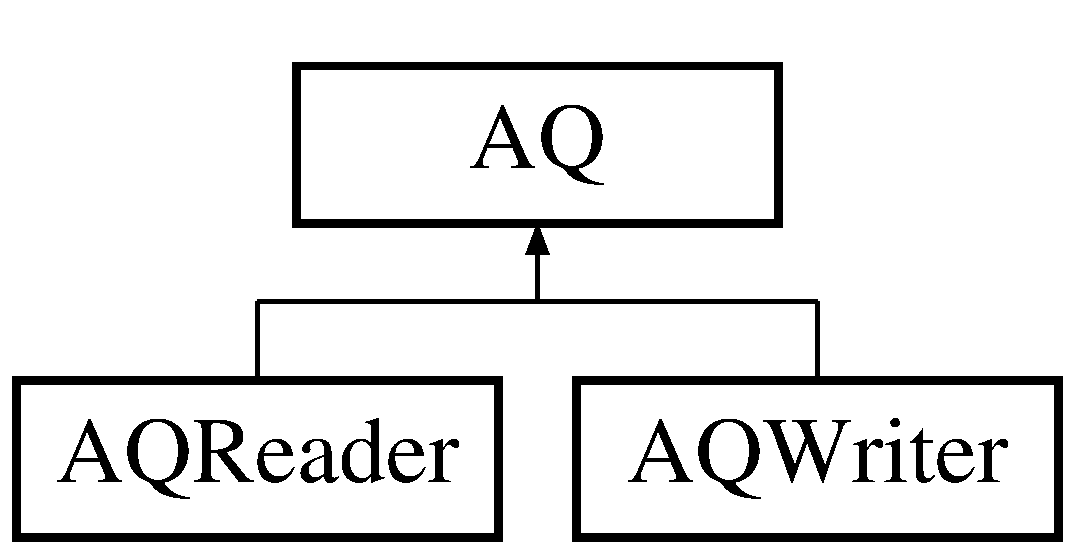
\includegraphics[height=2.000000cm]{class_a_q}
\end{center}
\end{figure}
\subsection*{Public Member Functions}
\begin{DoxyCompactItemize}
\item 
bool {\bfseries is\+Formatted} (void) const \hypertarget{class_a_q_a40ff86ec57b5e791b7e20c14e372999f}{}\label{class_a_q_a40ff86ec57b5e791b7e20c14e372999f}

\item 
bool {\bfseries is\+Extendable} (void) const \hypertarget{class_a_q_a7d869cae253ba0b35bd92cb38f647fda}{}\label{class_a_q_a7d869cae253ba0b35bd92cb38f647fda}

\item 
size\+\_\+t {\bfseries memory\+Size} (void) const \hypertarget{class_a_q_ae7442a5014d898f1f62f77737ce24feb}{}\label{class_a_q_ae7442a5014d898f1f62f77737ce24feb}

\item 
size\+\_\+t {\bfseries page\+Size} (void) const \hypertarget{class_a_q_ab47a5c88e8a23ec7a6e05f6d833c7d01}{}\label{class_a_q_ab47a5c88e8a23ec7a6e05f6d833c7d01}

\item 
size\+\_\+t {\bfseries page\+Count} (void) const \hypertarget{class_a_q_a0ee7e5627bf61ece4b47712d363aaeb9}{}\label{class_a_q_a0ee7e5627bf61ece4b47712d363aaeb9}

\item 
size\+\_\+t {\bfseries available\+Size} (void) const \hypertarget{class_a_q_a526b75b1f633fc6f96b6591ff47ef515}{}\label{class_a_q_a526b75b1f633fc6f96b6591ff47ef515}

\item 
uint32\+\_\+t {\bfseries claim\+Contention\+Count} (void) const \hypertarget{class_a_q_a83b0ae9501fdbc209a26868ff4c64ac3}{}\label{class_a_q_a83b0ae9501fdbc209a26868ff4c64ac3}

\end{DoxyCompactItemize}
\subsection*{Static Public Attributes}
\begin{DoxyCompactItemize}
\item 
static const unsigned int {\bfseries O\+P\+T\+I\+O\+N\+\_\+\+C\+R\+C32} = 1 $<$$<$ 0\hypertarget{class_a_q_a101384170c5d0275284c17e058ba17bb}{}\label{class_a_q_a101384170c5d0275284c17e058ba17bb}

\item 
static const unsigned int {\bfseries O\+P\+T\+I\+O\+N\+\_\+\+L\+I\+N\+K\+\_\+\+I\+D\+E\+N\+T\+I\+F\+I\+ER} = 1 $<$$<$ 1\hypertarget{class_a_q_ac5589df9ddcdc04100228b318b330cfa}{}\label{class_a_q_ac5589df9ddcdc04100228b318b330cfa}

\item 
static const unsigned int {\bfseries O\+P\+T\+I\+O\+N\+\_\+\+E\+X\+T\+E\+N\+D\+A\+B\+LE} = 1 $<$$<$ 2\hypertarget{class_a_q_a17b341a79c5d883ae5394e3a3e2fa773}{}\label{class_a_q_a17b341a79c5d883ae5394e3a3e2fa773}

\end{DoxyCompactItemize}
\subsection*{Protected Member Functions}
\begin{DoxyCompactItemize}
\item 
{\bfseries AQ} (int test\+Point\+Count, void $\ast$mem, size\+\_\+t mem\+Size, aq\+::\+Trace\+Buffer $\ast$trace=N\+U\+LL)\hypertarget{class_a_q_a1224c839b22d8d405528251b57018acd}{}\label{class_a_q_a1224c839b22d8d405528251b57018acd}

\item 
{\bfseries AQ} (const \hyperlink{class_a_q}{AQ} \&other)\hypertarget{class_a_q_ae058986ab79880ddaa3a71e05ddff0ba}{}\label{class_a_q_ae058986ab79880ddaa3a71e05ddff0ba}

\item 
\hyperlink{class_a_q}{AQ} \& {\bfseries operator=} (const \hyperlink{class_a_q}{AQ} \&other)\hypertarget{class_a_q_a618fbcd16dbef0162f70b16cc9321cf3}{}\label{class_a_q_a618fbcd16dbef0162f70b16cc9321cf3}

\item 
aq\+::\+Ctrl\+Overlay $\ast$ {\bfseries ctrl\+Throw\+On\+Unformatted} (const char $\ast$func) const \hypertarget{class_a_q_aa8057fd6a37d806aeabc29ce629d96da}{}\label{class_a_q_aa8057fd6a37d806aeabc29ce629d96da}

\item 
void {\bfseries test\+Point} (int tp)\hypertarget{class_a_q_a6e6c0d99fce0e1158a2ed804b95e42e6}{}\label{class_a_q_a6e6c0d99fce0e1158a2ed804b95e42e6}

\end{DoxyCompactItemize}
\subsection*{Protected Attributes}
\begin{DoxyCompactItemize}
\item 
aq\+::\+Trace\+Buffer $\ast$ {\bfseries m\+\_\+trace}\hypertarget{class_a_q_ac495082150eee429fa69db42503740fc}{}\label{class_a_q_ac495082150eee429fa69db42503740fc}

\item 
aq\+::\+Ctrl\+Overlay $\ast$ {\bfseries m\+\_\+ctrl}\hypertarget{class_a_q_aff98da408bd5646a825ddd4a1ac09d8d}{}\label{class_a_q_aff98da408bd5646a825ddd4a1ac09d8d}

\item 
size\+\_\+t {\bfseries m\+\_\+mem\+Size}\hypertarget{class_a_q_a400bbc49f484b688dc54ff4cc158cf31}{}\label{class_a_q_a400bbc49f484b688dc54ff4cc158cf31}

\end{DoxyCompactItemize}
\subsection*{Friends}
\begin{DoxyCompactItemize}
\item 
class {\bfseries A\+Q\+Snapshot}\hypertarget{class_a_q_a2f333d9188156b1bd94bce1fa73a38e0}{}\label{class_a_q_a2f333d9188156b1bd94bce1fa73a38e0}

\item 
class {\bfseries aq\+::\+Trace\+Buffer}\hypertarget{class_a_q_aaaed3688bb4cfc2496b3204ca4388b6a}{}\label{class_a_q_aaaed3688bb4cfc2496b3204ca4388b6a}

\end{DoxyCompactItemize}


The documentation for this class was generated from the following files\+:\begin{DoxyCompactItemize}
\item 
A\+Q.\+h\item 
A\+Q.\+cpp\end{DoxyCompactItemize}

\hypertarget{class_a_q_item}{}\section{A\+Q\+Item Class Reference}
\label{class_a_q_item}\index{A\+Q\+Item@{A\+Q\+Item}}
Inheritance diagram for A\+Q\+Item\+:\begin{figure}[H]
\begin{center}
\leavevmode
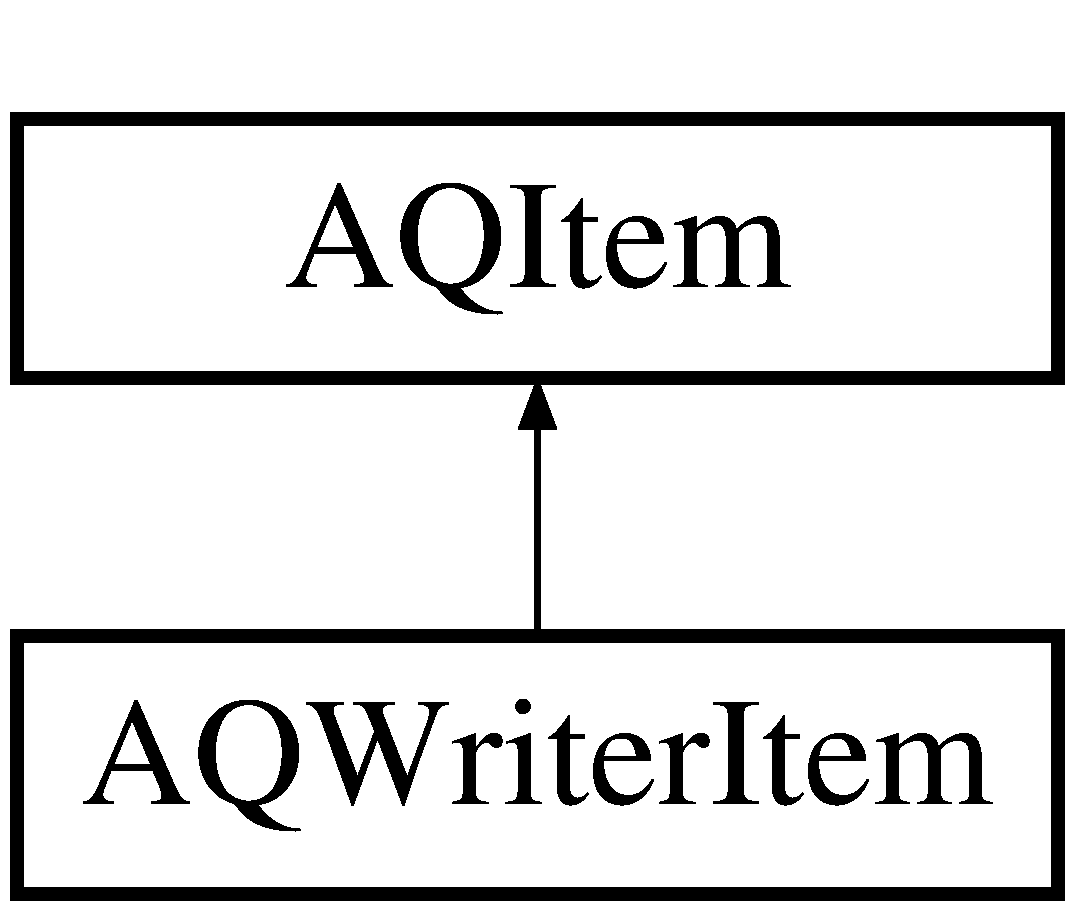
\includegraphics[height=2.000000cm]{class_a_q_item}
\end{center}
\end{figure}
\subsection*{Public Member Functions}
\begin{DoxyCompactItemize}
\item 
{\bfseries A\+Q\+Item} (const \hyperlink{class_a_q_item}{A\+Q\+Item} \&other)\hypertarget{class_a_q_item_a97f5c3ef3f493c5c6df7a2dd4cc0d4b5}{}\label{class_a_q_item_a97f5c3ef3f493c5c6df7a2dd4cc0d4b5}

\item 
\hyperlink{class_a_q_item}{A\+Q\+Item} \& {\bfseries operator=} (const \hyperlink{class_a_q_item}{A\+Q\+Item} \&other)\hypertarget{class_a_q_item_a780c92d7ed552d69ac2a692d09ca3a2b}{}\label{class_a_q_item_a780c92d7ed552d69ac2a692d09ca3a2b}

\item 
void {\bfseries clear} (void)\hypertarget{class_a_q_item_ae169220dd19f29c74d891935d2d9d4b8}{}\label{class_a_q_item_ae169220dd19f29c74d891935d2d9d4b8}

\item 
uint32\+\_\+t {\bfseries queue\+Identifier} (void) const \hypertarget{class_a_q_item_a33029e27ef81601694a987648cd09f67}{}\label{class_a_q_item_a33029e27ef81601694a987648cd09f67}

\item 
uint32\+\_\+t {\bfseries link\+Identifier} (void) const \hypertarget{class_a_q_item_a8e2e1414d09863cf3b733119a068dbb8}{}\label{class_a_q_item_a8e2e1414d09863cf3b733119a068dbb8}

\item 
bool {\bfseries is\+Allocated} (void) const \hypertarget{class_a_q_item_a21513e2a0208dbbd000c1821913ff595}{}\label{class_a_q_item_a21513e2a0208dbbd000c1821913ff595}

\item 
bool {\bfseries is\+Committed} (void) const \hypertarget{class_a_q_item_a09f66df9383cbeec05990270d2517397}{}\label{class_a_q_item_a09f66df9383cbeec05990270d2517397}

\item 
bool {\bfseries is\+Released} (void) const \hypertarget{class_a_q_item_ac3eb62c6b4c6dee0c2afafafd8bea06f}{}\label{class_a_q_item_ac3eb62c6b4c6dee0c2afafafd8bea06f}

\item 
bool {\bfseries is\+Checksum\+Valid} (void) const \hypertarget{class_a_q_item_a2313675d412d90c4b54da718dbd487fc}{}\label{class_a_q_item_a2313675d412d90c4b54da718dbd487fc}

\item 
size\+\_\+t {\bfseries size} (void) const \hypertarget{class_a_q_item_a346237d15617f812d325c173f21892b9}{}\label{class_a_q_item_a346237d15617f812d325c173f21892b9}

\item 
size\+\_\+t {\bfseries capacity} (void) const \hypertarget{class_a_q_item_aba43b837efe456e423cf290b7bdae608}{}\label{class_a_q_item_aba43b837efe456e423cf290b7bdae608}

\item 
const unsigned char \& {\bfseries operator\mbox{[}$\,$\mbox{]}} (size\+\_\+t idx) const \hypertarget{class_a_q_item_a395900d5781030372dfc231d2361d41c}{}\label{class_a_q_item_a395900d5781030372dfc231d2361d41c}

\item 
const \hyperlink{class_a_q_item}{A\+Q\+Item} $\ast$ {\bfseries first} (void) const \hypertarget{class_a_q_item_ab109099474cb358ce7b2cd0cbbf4a530}{}\label{class_a_q_item_ab109099474cb358ce7b2cd0cbbf4a530}

\item 
const \hyperlink{class_a_q_item}{A\+Q\+Item} $\ast$ {\bfseries last} (void) const \hypertarget{class_a_q_item_a71b8a01fb113490f2c96bf9a7cf60e8c}{}\label{class_a_q_item_a71b8a01fb113490f2c96bf9a7cf60e8c}

\item 
const \hyperlink{class_a_q_item}{A\+Q\+Item} $\ast$ {\bfseries next} (void) const \hypertarget{class_a_q_item_a852962115eaa0b0bd8d356a682778afe}{}\label{class_a_q_item_a852962115eaa0b0bd8d356a682778afe}

\item 
const \hyperlink{class_a_q_item}{A\+Q\+Item} $\ast$ {\bfseries prev} (void) const \hypertarget{class_a_q_item_a5afdc65d0570f2ee4bac6c3d61c2e16f}{}\label{class_a_q_item_a5afdc65d0570f2ee4bac6c3d61c2e16f}

\end{DoxyCompactItemize}
\subsection*{Static Public Attributes}
\begin{DoxyCompactItemize}
\item 
static const uint32\+\_\+t {\bfseries Q\+U\+E\+U\+E\+\_\+\+I\+D\+E\+N\+T\+I\+F\+I\+E\+R\+\_\+\+M\+A\+SK} = 0x1\+F\+F\+F\+F\+F\+FF\hypertarget{class_a_q_item_aaa5f97ad56a729c0ae1e8687111a9a40}{}\label{class_a_q_item_aaa5f97ad56a729c0ae1e8687111a9a40}

\item 
static const uint32\+\_\+t {\bfseries Q\+U\+E\+U\+E\+\_\+\+I\+D\+E\+N\+T\+I\+F\+I\+E\+R\+\_\+\+U\+S\+E\+R\+\_\+\+M\+A\+SK} = 0x\+E0000000\hypertarget{class_a_q_item_a535cc166babbb9927ed075dc08eddaba}{}\label{class_a_q_item_a535cc166babbb9927ed075dc08eddaba}

\item 
static const uint32\+\_\+t {\bfseries Q\+U\+E\+U\+E\+\_\+\+I\+D\+E\+N\+T\+I\+F\+I\+E\+R\+\_\+\+U\+S\+E\+R\+\_\+\+B\+IT} = 29\hypertarget{class_a_q_item_a53a0322677680ab691ff049dc69a2aa1}{}\label{class_a_q_item_a53a0322677680ab691ff049dc69a2aa1}

\item 
static const uint32\+\_\+t {\bfseries Q\+U\+E\+U\+E\+\_\+\+I\+D\+E\+N\+T\+I\+F\+I\+E\+R\+\_\+\+I\+N\+V\+A\+L\+ID} = 0x\+F\+F\+F\+F\+F\+F\+FF\hypertarget{class_a_q_item_a987fe89fa76ce1733f1f8146873aead8}{}\label{class_a_q_item_a987fe89fa76ce1733f1f8146873aead8}

\end{DoxyCompactItemize}
\subsection*{Protected Member Functions}
\begin{DoxyCompactItemize}
\item 
virtual \hyperlink{class_a_q_item}{A\+Q\+Item} $\ast$ {\bfseries new\+Instance} (void) const \hypertarget{class_a_q_item_a998267c4e39d73e23e3740189f0ba884}{}\label{class_a_q_item_a998267c4e39d73e23e3740189f0ba884}

\item 
unsigned char $\ast$ {\bfseries mem} (void) const \hypertarget{class_a_q_item_ad66cddfab0d74ef3de890a915631d3b7}{}\label{class_a_q_item_ad66cddfab0d74ef3de890a915631d3b7}

\item 
uint32\+\_\+t {\bfseries ctrl} (void) const \hypertarget{class_a_q_item_a8815e7003fabbf8ab3462f8d570c0414}{}\label{class_a_q_item_a8815e7003fabbf8ab3462f8d570c0414}

\end{DoxyCompactItemize}
\subsection*{Protected Attributes}
\begin{DoxyCompactItemize}
\item 
unsigned char $\ast$ {\bfseries m\+\_\+mem}\hypertarget{class_a_q_item_ac5ea4955cd4231d3c378d7660798da22}{}\label{class_a_q_item_ac5ea4955cd4231d3c378d7660798da22}

\item 
size\+\_\+t {\bfseries m\+\_\+mem\+Size}\hypertarget{class_a_q_item_a4e58e13e55d38e68f7d30b10bf998103}{}\label{class_a_q_item_a4e58e13e55d38e68f7d30b10bf998103}

\item 
\hyperlink{class_a_q_item}{A\+Q\+Item} $\ast$ {\bfseries m\+\_\+first}\hypertarget{class_a_q_item_a2d6f7457dac6d0103ac4559717d89848}{}\label{class_a_q_item_a2d6f7457dac6d0103ac4559717d89848}

\item 
\hyperlink{class_a_q_item}{A\+Q\+Item} $\ast$ {\bfseries m\+\_\+next}\hypertarget{class_a_q_item_a9af0456439904c17603c758033665a74}{}\label{class_a_q_item_a9af0456439904c17603c758033665a74}

\item 
\hyperlink{class_a_q_item}{A\+Q\+Item} $\ast$ {\bfseries m\+\_\+prev}\hypertarget{class_a_q_item_a140794796d543ba3cd00f081059f9f8f}{}\label{class_a_q_item_a140794796d543ba3cd00f081059f9f8f}

\item 
uint32\+\_\+t {\bfseries m\+\_\+lkid}\hypertarget{class_a_q_item_a442666d251ed4f17ac8957fe9ddad1e5}{}\label{class_a_q_item_a442666d251ed4f17ac8957fe9ddad1e5}

\end{DoxyCompactItemize}
\subsection*{Friends}
\begin{DoxyCompactItemize}
\item 
class {\bfseries A\+Q\+Reader}\hypertarget{class_a_q_item_a846a72114e5337de444fd4ef617e8fc2}{}\label{class_a_q_item_a846a72114e5337de444fd4ef617e8fc2}

\item 
class {\bfseries A\+Q\+Writer}\hypertarget{class_a_q_item_af06d9ff3c550f5e56ca5f6ca0c12db6c}{}\label{class_a_q_item_af06d9ff3c550f5e56ca5f6ca0c12db6c}

\item 
class {\bfseries X\+A\+Q\+Reader}\hypertarget{class_a_q_item_a2f01ef455aefd09d46a49746262759d2}{}\label{class_a_q_item_a2f01ef455aefd09d46a49746262759d2}

\item 
class {\bfseries X\+A\+Q\+Writer}\hypertarget{class_a_q_item_a50c9367cbf2f427d33949023a0ec4c96}{}\label{class_a_q_item_a50c9367cbf2f427d33949023a0ec4c96}

\item 
class {\bfseries A\+Q\+Snapshot}\hypertarget{class_a_q_item_a2f333d9188156b1bd94bce1fa73a38e0}{}\label{class_a_q_item_a2f333d9188156b1bd94bce1fa73a38e0}

\item 
class {\bfseries aq\+::\+Trace\+Buffer}\hypertarget{class_a_q_item_aaaed3688bb4cfc2496b3204ca4388b6a}{}\label{class_a_q_item_aaaed3688bb4cfc2496b3204ca4388b6a}

\item 
class {\bfseries aq\+::\+Linked\+Item\+Processor}\hypertarget{class_a_q_item_a726d915ae4e0c3576ddb9a3899d76d0b}{}\label{class_a_q_item_a726d915ae4e0c3576ddb9a3899d76d0b}

\item 
class {\bfseries A\+Q\+Test}\hypertarget{class_a_q_item_ac28a91f88be754d785cda9b1b23fb17d}{}\label{class_a_q_item_ac28a91f88be754d785cda9b1b23fb17d}

\item 
class {\bfseries A\+Q\+Straw\+Man\+Base}\hypertarget{class_a_q_item_a6db0b94f3c31d8a168937c85eb81515f}{}\label{class_a_q_item_a6db0b94f3c31d8a168937c85eb81515f}

\end{DoxyCompactItemize}


The documentation for this class was generated from the following files\+:\begin{DoxyCompactItemize}
\item 
A\+Q\+Item.\+h\item 
A\+Q\+Item.\+cpp\end{DoxyCompactItemize}

\hypertarget{class_a_q_reader}{}\section{A\+Q\+Reader Class Reference}
\label{class_a_q_reader}\index{A\+Q\+Reader@{A\+Q\+Reader}}
Inheritance diagram for A\+Q\+Reader\+:\begin{figure}[H]
\begin{center}
\leavevmode
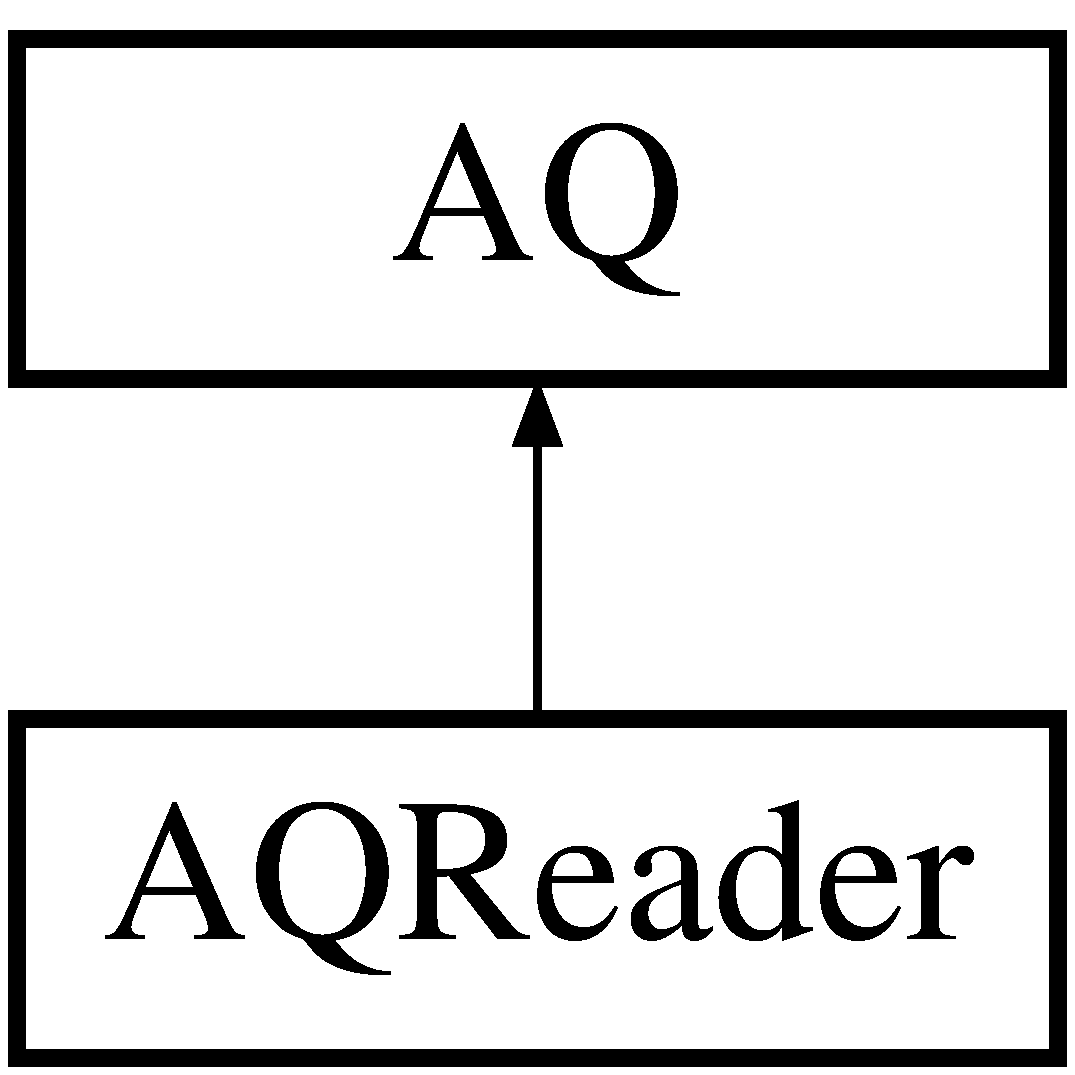
\includegraphics[height=2.000000cm]{class_a_q_reader}
\end{center}
\end{figure}
\subsection*{Public Member Functions}
\begin{DoxyCompactItemize}
\item 
{\bfseries A\+Q\+Reader} (void $\ast$mem, size\+\_\+t mem\+Sz, aq\+::\+Trace\+Buffer $\ast$trace=N\+U\+LL)\hypertarget{class_a_q_reader_a58e6ba2ed65f3b6ea6e324d85662726a}{}\label{class_a_q_reader_a58e6ba2ed65f3b6ea6e324d85662726a}

\item 
{\bfseries A\+Q\+Reader} (const \hyperlink{class_a_q_reader}{A\+Q\+Reader} \&other)\hypertarget{class_a_q_reader_a7f8e630340547a340e5244e7c19dbbc4}{}\label{class_a_q_reader_a7f8e630340547a340e5244e7c19dbbc4}

\item 
\hyperlink{class_a_q_reader}{A\+Q\+Reader} \& {\bfseries operator=} (const \hyperlink{class_a_q_reader}{A\+Q\+Reader} \&other)\hypertarget{class_a_q_reader_a9fa06085b152d9587102216114c13e4a}{}\label{class_a_q_reader_a9fa06085b152d9587102216114c13e4a}

\item 
bool {\bfseries format} (int page\+Size\+Shift, unsigned int commit\+Timeout\+Ms, unsigned int options=0)\hypertarget{class_a_q_reader_ac9bcc041a825dc8f3d57d9644ea65863}{}\label{class_a_q_reader_ac9bcc041a825dc8f3d57d9644ea65863}

\item 
const volatile uint32\+\_\+t \& {\bfseries commit\+Counter} (void) const \hypertarget{class_a_q_reader_a97babb3a8853758a2c37c68ecd27fe3f}{}\label{class_a_q_reader_a97babb3a8853758a2c37c68ecd27fe3f}

\item 
bool {\bfseries retrieve} (\hyperlink{class_a_q_item}{A\+Q\+Item} \&item)\hypertarget{class_a_q_reader_a6746d86b29c04ff19032106323cdef6f}{}\label{class_a_q_reader_a6746d86b29c04ff19032106323cdef6f}

\item 
void {\bfseries release} (\hyperlink{class_a_q_item}{A\+Q\+Item} \&item)\hypertarget{class_a_q_reader_aad5233986e056a2da7f23e282b7a2596}{}\label{class_a_q_reader_aad5233986e056a2da7f23e282b7a2596}

\item 
void {\bfseries release\+Extendable} (\hyperlink{class_a_q_item}{A\+Q\+Item} \&item, size\+\_\+t start, size\+\_\+t end)\hypertarget{class_a_q_reader_a67bfd41350cadc6af749df9132a0901c}{}\label{class_a_q_reader_a67bfd41350cadc6af749df9132a0901c}

\end{DoxyCompactItemize}
\subsection*{Static Public Attributes}
\begin{DoxyCompactItemize}
\item 
static const int {\bfseries Release\+Before\+Write\+Second\+Ctrl} = 0\hypertarget{class_a_q_reader_afc4fc5bc47126f689f250633e696b974}{}\label{class_a_q_reader_afc4fc5bc47126f689f250633e696b974}

\item 
static const int {\bfseries Walk\+Before\+Write\+Ctrl} = Release\+Before\+Write\+Second\+Ctrl + 1\hypertarget{class_a_q_reader_ad1bea8ce5f71051ab9e08a7082b5c47a}{}\label{class_a_q_reader_ad1bea8ce5f71051ab9e08a7082b5c47a}

\item 
static const int {\bfseries Walk\+Before\+Write\+Tail\+Ref} = Walk\+Before\+Write\+Ctrl + 1\hypertarget{class_a_q_reader_a49a0d882ae89a520a0c32ca407172e33}{}\label{class_a_q_reader_a49a0d882ae89a520a0c32ca407172e33}

\item 
static const int {\bfseries Walk\+After\+Read\+CtrlN} = Walk\+Before\+Write\+Tail\+Ref + 1\hypertarget{class_a_q_reader_a82f7a6e5151119edaddcd0ccc167547b}{}\label{class_a_q_reader_a82f7a6e5151119edaddcd0ccc167547b}

\item 
static const int {\bfseries Test\+Point\+Count} = Walk\+After\+Read\+CtrlN + 11\hypertarget{class_a_q_reader_a3d1f81f5acfd2b55b226d2545fc9d9f1}{}\label{class_a_q_reader_a3d1f81f5acfd2b55b226d2545fc9d9f1}

\end{DoxyCompactItemize}
\subsection*{Additional Inherited Members}


The documentation for this class was generated from the following files\+:\begin{DoxyCompactItemize}
\item 
A\+Q\+Reader.\+h\item 
A\+Q\+Reader.\+cpp\end{DoxyCompactItemize}

\hypertarget{class_a_q_snapshot}{}\section{A\+Q\+Snapshot Class Reference}
\label{class_a_q_snapshot}\index{A\+Q\+Snapshot@{A\+Q\+Snapshot}}
\subsection*{Public Member Functions}
\begin{DoxyCompactItemize}
\item 
{\bfseries A\+Q\+Snapshot} (aq\+::\+Trace\+Buffer $\ast$trace=N\+U\+LL)\hypertarget{class_a_q_snapshot_a95d65f0f166eaaeaf321dc66df231366}{}\label{class_a_q_snapshot_a95d65f0f166eaaeaf321dc66df231366}

\item 
{\bfseries A\+Q\+Snapshot} (const \hyperlink{class_a_q}{AQ} \&queue, aq\+::\+Trace\+Buffer $\ast$trace=N\+U\+LL)\hypertarget{class_a_q_snapshot_acd641f8ba5493df284cc09b546ffe687}{}\label{class_a_q_snapshot_acd641f8ba5493df284cc09b546ffe687}

\item 
{\bfseries A\+Q\+Snapshot} (const \hyperlink{class_a_q_snapshot}{A\+Q\+Snapshot} \&other)\hypertarget{class_a_q_snapshot_aeee8da6b40d706aadcdfc191502d8e7e}{}\label{class_a_q_snapshot_aeee8da6b40d706aadcdfc191502d8e7e}

\item 
\hyperlink{class_a_q_snapshot}{A\+Q\+Snapshot} \& {\bfseries operator=} (const \hyperlink{class_a_q_snapshot}{A\+Q\+Snapshot} \&other)\hypertarget{class_a_q_snapshot_a901ac5ebb680f56f4d3a305e15db7b4f}{}\label{class_a_q_snapshot_a901ac5ebb680f56f4d3a305e15db7b4f}

\item 
void {\bfseries snap} (const \hyperlink{class_a_q}{AQ} \&queue)\hypertarget{class_a_q_snapshot_a60d0ddba6b37297f349db12f1f8fdd21}{}\label{class_a_q_snapshot_a60d0ddba6b37297f349db12f1f8fdd21}

\item 
void {\bfseries snap1\+Initial\+Head} (const \hyperlink{class_a_q}{AQ} \&queue)\hypertarget{class_a_q_snapshot_ac96df72098fc41dfb0750e4f9bdf8da3}{}\label{class_a_q_snapshot_ac96df72098fc41dfb0750e4f9bdf8da3}

\item 
void {\bfseries snap2\+Initial\+Ctrlq} (void)\hypertarget{class_a_q_snapshot_a7f435e4d7d57bf75c027274c5a735a26}{}\label{class_a_q_snapshot_a7f435e4d7d57bf75c027274c5a735a26}

\item 
void {\bfseries snap3\+Page\+Memory} (void)\hypertarget{class_a_q_snapshot_af6678e323b473546ff0c3897eee9c9a4}{}\label{class_a_q_snapshot_af6678e323b473546ff0c3897eee9c9a4}

\item 
void {\bfseries snap4\+Final\+Head} (void)\hypertarget{class_a_q_snapshot_ad9441788c37ebc61eedd38a5bd05aa01}{}\label{class_a_q_snapshot_ad9441788c37ebc61eedd38a5bd05aa01}

\item 
uint32\+\_\+t {\bfseries init\+Head\+Ref} (void) const \hypertarget{class_a_q_snapshot_a5ee63bb9f5ef210057ffdfaa61b1875d}{}\label{class_a_q_snapshot_a5ee63bb9f5ef210057ffdfaa61b1875d}

\item 
uint32\+\_\+t {\bfseries final\+Head\+Ref} (void) const \hypertarget{class_a_q_snapshot_a22e3bcff55f5739df18a2db3e13180e9}{}\label{class_a_q_snapshot_a22e3bcff55f5739df18a2db3e13180e9}

\item 
size\+\_\+t {\bfseries size} (void) const \hypertarget{class_a_q_snapshot_a951996216da0d1fc84f9d923620ba1af}{}\label{class_a_q_snapshot_a951996216da0d1fc84f9d923620ba1af}

\item 
const \hyperlink{class_a_q_item}{A\+Q\+Item} \& {\bfseries operator\mbox{[}$\,$\mbox{]}} (size\+\_\+t idx) const \hypertarget{class_a_q_snapshot_ad2b0f8616beab3e8fd012031a712bd0a}{}\label{class_a_q_snapshot_ad2b0f8616beab3e8fd012031a712bd0a}

\end{DoxyCompactItemize}


The documentation for this class was generated from the following files\+:\begin{DoxyCompactItemize}
\item 
A\+Q\+Snapshot.\+h\item 
A\+Q\+Snapshot.\+cpp\end{DoxyCompactItemize}

\hypertarget{class_a_q_unformatted_exception}{}\section{A\+Q\+Unformatted\+Exception Class Reference}
\label{class_a_q_unformatted_exception}\index{A\+Q\+Unformatted\+Exception@{A\+Q\+Unformatted\+Exception}}
Inheritance diagram for A\+Q\+Unformatted\+Exception\+:\begin{figure}[H]
\begin{center}
\leavevmode
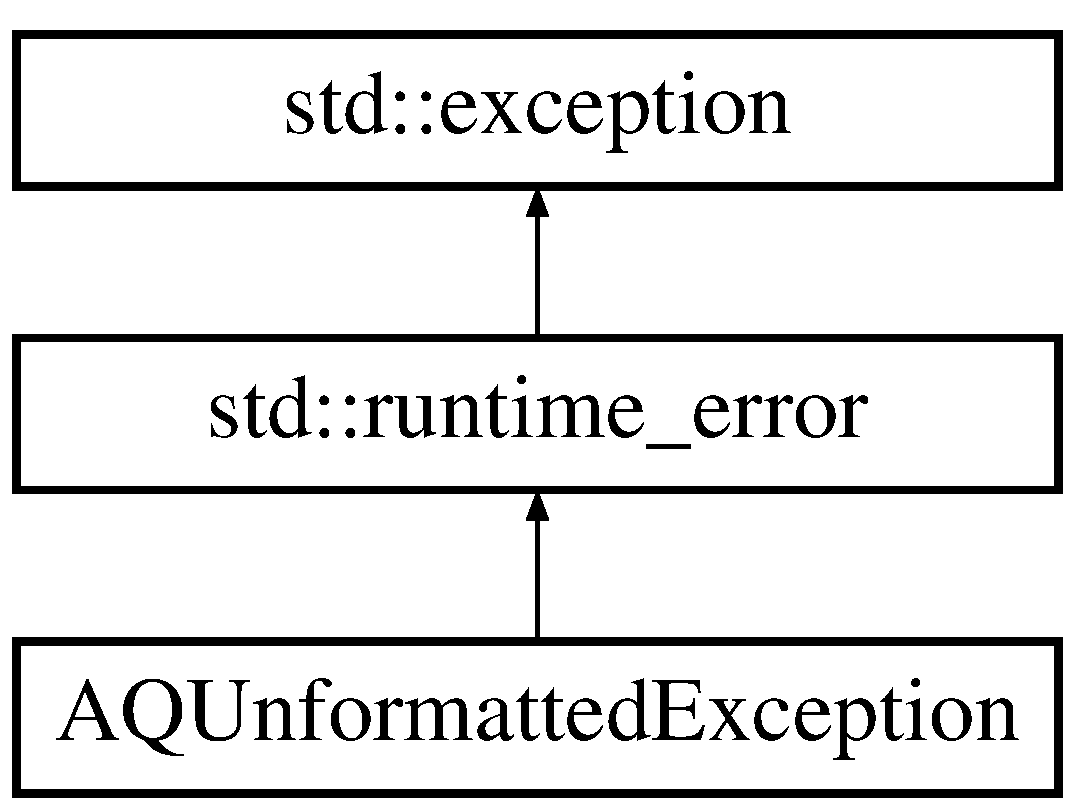
\includegraphics[height=3.000000cm]{class_a_q_unformatted_exception}
\end{center}
\end{figure}
\subsection*{Public Member Functions}
\begin{DoxyCompactItemize}
\item 
{\bfseries A\+Q\+Unformatted\+Exception} (const std\+::string \&msg)\hypertarget{class_a_q_unformatted_exception_a61ea812823c79cde5c1ce12624af453e}{}\label{class_a_q_unformatted_exception_a61ea812823c79cde5c1ce12624af453e}

\item 
{\bfseries A\+Q\+Unformatted\+Exception} (const \hyperlink{class_a_q_unformatted_exception}{A\+Q\+Unformatted\+Exception} \&other)\hypertarget{class_a_q_unformatted_exception_a80cac0b2a15cf523c52955198cebf463}{}\label{class_a_q_unformatted_exception_a80cac0b2a15cf523c52955198cebf463}

\item 
\hyperlink{class_a_q_unformatted_exception}{A\+Q\+Unformatted\+Exception} \& {\bfseries operator=} (const \hyperlink{class_a_q_unformatted_exception}{A\+Q\+Unformatted\+Exception} \&other)\hypertarget{class_a_q_unformatted_exception_ae68d1b7ff69dd77f0952598269129912}{}\label{class_a_q_unformatted_exception_ae68d1b7ff69dd77f0952598269129912}

\end{DoxyCompactItemize}


The documentation for this class was generated from the following files\+:\begin{DoxyCompactItemize}
\item 
A\+Q\+Unformatted\+Exception.\+h\item 
A\+Q\+Unformatted\+Exception.\+cpp\end{DoxyCompactItemize}

\hypertarget{class_a_q_writer}{}\section{A\+Q\+Writer Class Reference}
\label{class_a_q_writer}\index{A\+Q\+Writer@{A\+Q\+Writer}}
Inheritance diagram for A\+Q\+Writer\+:\begin{figure}[H]
\begin{center}
\leavevmode
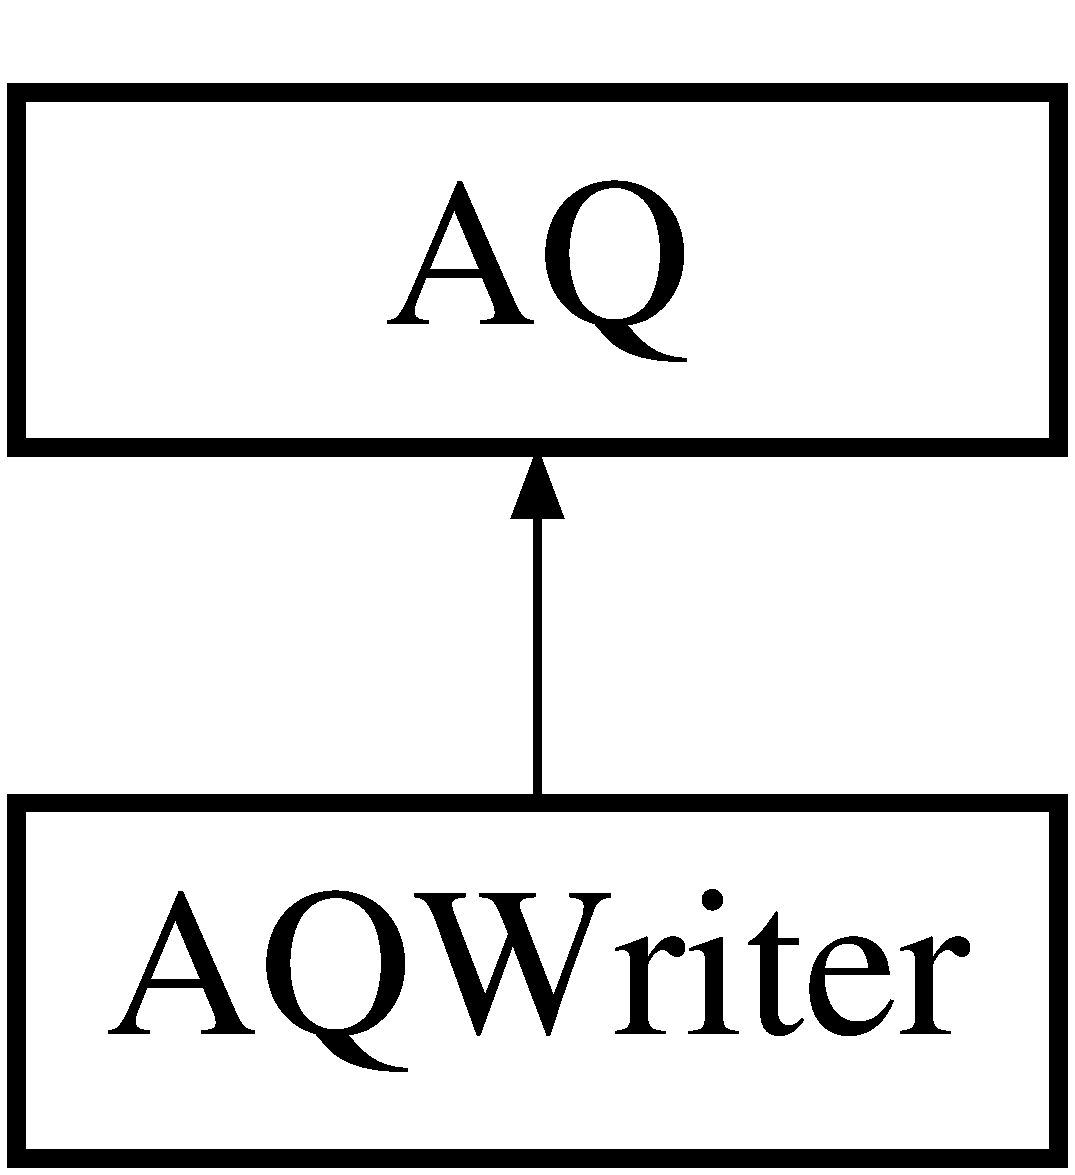
\includegraphics[height=2.000000cm]{class_a_q_writer}
\end{center}
\end{figure}
\subsection*{Public Member Functions}
\begin{DoxyCompactItemize}
\item 
{\bfseries A\+Q\+Writer} (void $\ast$mem, size\+\_\+t mem\+Size, aq\+::\+Trace\+Buffer $\ast$trace=N\+U\+LL)\hypertarget{class_a_q_writer_af0b7130d88826565128ff5c52451d095}{}\label{class_a_q_writer_af0b7130d88826565128ff5c52451d095}

\item 
{\bfseries A\+Q\+Writer} (const \hyperlink{class_a_q_writer}{A\+Q\+Writer} \&other)\hypertarget{class_a_q_writer_adfec5d995bc6262d4381e630aae16bea}{}\label{class_a_q_writer_adfec5d995bc6262d4381e630aae16bea}

\item 
\hyperlink{class_a_q_writer}{A\+Q\+Writer} \& {\bfseries operator=} (const \hyperlink{class_a_q_writer}{A\+Q\+Writer} \&other)\hypertarget{class_a_q_writer_a4f1d7b7322b0e47b2573f2ba7da844ed}{}\label{class_a_q_writer_a4f1d7b7322b0e47b2573f2ba7da844ed}

\item 
const volatile uint32\+\_\+t \& {\bfseries free\+Counter} (void) const \hypertarget{class_a_q_writer_a6eb5b715a284fc141a8671ebee3bd293}{}\label{class_a_q_writer_a6eb5b715a284fc141a8671ebee3bd293}

\item 
bool {\bfseries claim} (\hyperlink{class_a_q_writer_item}{A\+Q\+Writer\+Item} \&item, size\+\_\+t mem\+Size)\hypertarget{class_a_q_writer_ae0e2eeac326abd648b6aa60a1fb5315a}{}\label{class_a_q_writer_ae0e2eeac326abd648b6aa60a1fb5315a}

\item 
bool {\bfseries commit} (\hyperlink{class_a_q_writer_item}{A\+Q\+Writer\+Item} \&item)\hypertarget{class_a_q_writer_a598bba1f79e007e038ab76d8939a5b56}{}\label{class_a_q_writer_a598bba1f79e007e038ab76d8939a5b56}

\item 
bool {\bfseries commit\+Extendable} (\hyperlink{class_a_q_writer_item}{A\+Q\+Writer\+Item} \&item, size\+\_\+t start, size\+\_\+t end)\hypertarget{class_a_q_writer_a74fddc416d47cac08b87a9032a8ca2ce}{}\label{class_a_q_writer_a74fddc416d47cac08b87a9032a8ca2ce}

\end{DoxyCompactItemize}
\subsection*{Static Public Attributes}
\begin{DoxyCompactItemize}
\item 
static const int {\bfseries Claim\+Before\+Write\+Head\+Ref} = 0\hypertarget{class_a_q_writer_a3074dbe598b3a940d6ff60a0d4e2edd2}{}\label{class_a_q_writer_a3074dbe598b3a940d6ff60a0d4e2edd2}

\item 
static const int {\bfseries Claim\+Before\+Write\+Ctrl\+Skip\+Pages} = Claim\+Before\+Write\+Head\+Ref + 1\hypertarget{class_a_q_writer_a025b95cc9c443b0869389b89dbd0f174}{}\label{class_a_q_writer_a025b95cc9c443b0869389b89dbd0f174}

\item 
static const int {\bfseries Claim\+Before\+Write\+Ctrl} = Claim\+Before\+Write\+Ctrl\+Skip\+Pages + 1\hypertarget{class_a_q_writer_a18ec1b67b267790fe9fceb79a9fbf7b7}{}\label{class_a_q_writer_a18ec1b67b267790fe9fceb79a9fbf7b7}

\item 
static const int {\bfseries Commit\+Before\+Write\+Ctrl} = Claim\+Before\+Write\+Ctrl + 1\hypertarget{class_a_q_writer_a2057ecc1b059fcba2b5497fcfce4c104}{}\label{class_a_q_writer_a2057ecc1b059fcba2b5497fcfce4c104}

\item 
static const int {\bfseries Test\+Point\+Count} = Commit\+Before\+Write\+Ctrl + 1\hypertarget{class_a_q_writer_a8d574c3551be31f6ff288fd4757210ba}{}\label{class_a_q_writer_a8d574c3551be31f6ff288fd4757210ba}

\end{DoxyCompactItemize}
\subsection*{Additional Inherited Members}


The documentation for this class was generated from the following files\+:\begin{DoxyCompactItemize}
\item 
A\+Q\+Writer.\+h\item 
A\+Q\+Writer.\+cpp\end{DoxyCompactItemize}

\hypertarget{class_a_q_writer_item}{}\section{A\+Q\+Writer\+Item Class Reference}
\label{class_a_q_writer_item}\index{A\+Q\+Writer\+Item@{A\+Q\+Writer\+Item}}
Inheritance diagram for A\+Q\+Writer\+Item\+:\begin{figure}[H]
\begin{center}
\leavevmode
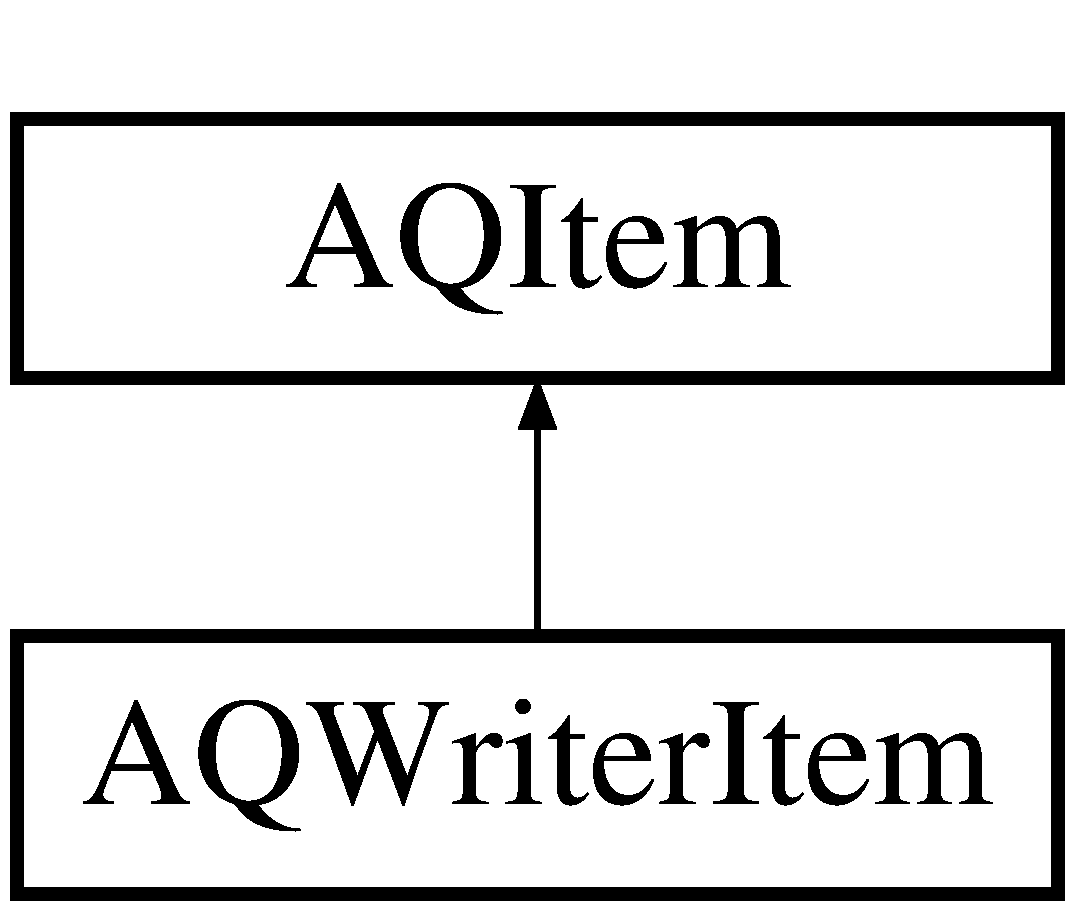
\includegraphics[height=2.000000cm]{class_a_q_writer_item}
\end{center}
\end{figure}
\subsection*{Public Member Functions}
\begin{DoxyCompactItemize}
\item 
{\bfseries A\+Q\+Writer\+Item} (const \hyperlink{class_a_q_writer_item}{A\+Q\+Writer\+Item} \&other)\hypertarget{class_a_q_writer_item_afb89ea3ad90a751066342f136fe4b2fd}{}\label{class_a_q_writer_item_afb89ea3ad90a751066342f136fe4b2fd}

\item 
\hyperlink{class_a_q_writer_item}{A\+Q\+Writer\+Item} \& {\bfseries operator=} (const \hyperlink{class_a_q_writer_item}{A\+Q\+Writer\+Item} \&other)\hypertarget{class_a_q_writer_item_a626754df58bf7442942ffcde296aac36}{}\label{class_a_q_writer_item_a626754df58bf7442942ffcde296aac36}

\item 
void {\bfseries set\+Link\+Identifier} (uint32\+\_\+t lkid)\hypertarget{class_a_q_writer_item_a52f19448fb3ca5fd9e1afbeb7d60027a}{}\label{class_a_q_writer_item_a52f19448fb3ca5fd9e1afbeb7d60027a}

\item 
const unsigned char \& {\bfseries operator\mbox{[}$\,$\mbox{]}} (size\+\_\+t idx) const \hypertarget{class_a_q_writer_item_ab025ce2d8f8ec5716b97a6d8cfd6056a}{}\label{class_a_q_writer_item_ab025ce2d8f8ec5716b97a6d8cfd6056a}

\item 
unsigned char \& {\bfseries operator\mbox{[}$\,$\mbox{]}} (size\+\_\+t idx)\hypertarget{class_a_q_writer_item_a4b1cf82c67ef0f1aa6a52786124d2d64}{}\label{class_a_q_writer_item_a4b1cf82c67ef0f1aa6a52786124d2d64}

\item 
bool {\bfseries write} (const void $\ast$mem, size\+\_\+t mem\+Size)\hypertarget{class_a_q_writer_item_a06d5dcc6535fbbc3f06bc2a56ed2ae18}{}\label{class_a_q_writer_item_a06d5dcc6535fbbc3f06bc2a56ed2ae18}

\item 
bool {\bfseries write} (size\+\_\+t off, const void $\ast$mem, size\+\_\+t mem\+Size)\hypertarget{class_a_q_writer_item_a108cb5fa1ed80fd8dab609581283010d}{}\label{class_a_q_writer_item_a108cb5fa1ed80fd8dab609581283010d}

\item 
\hyperlink{class_a_q_writer_item}{A\+Q\+Writer\+Item} $\ast$ {\bfseries first} (void)\hypertarget{class_a_q_writer_item_a8efccaf791f519033681a23cbce1ed0a}{}\label{class_a_q_writer_item_a8efccaf791f519033681a23cbce1ed0a}

\item 
\hyperlink{class_a_q_writer_item}{A\+Q\+Writer\+Item} $\ast$ {\bfseries last} (void)\hypertarget{class_a_q_writer_item_aeaa1e6bdd9019370b253029f5c09c802}{}\label{class_a_q_writer_item_aeaa1e6bdd9019370b253029f5c09c802}

\item 
\hyperlink{class_a_q_writer_item}{A\+Q\+Writer\+Item} $\ast$ {\bfseries next} (void)\hypertarget{class_a_q_writer_item_a8615aa9e620aac3ece8c2512b6c25c5c}{}\label{class_a_q_writer_item_a8615aa9e620aac3ece8c2512b6c25c5c}

\item 
\hyperlink{class_a_q_writer_item}{A\+Q\+Writer\+Item} $\ast$ {\bfseries prev} (void)\hypertarget{class_a_q_writer_item_ad8a7fb46a46fb9205e1d653502e07c7f}{}\label{class_a_q_writer_item_ad8a7fb46a46fb9205e1d653502e07c7f}

\item 
const \hyperlink{class_a_q_writer_item}{A\+Q\+Writer\+Item} $\ast$ {\bfseries first} (void) const \hypertarget{class_a_q_writer_item_a20ad481c8956678a122c39f921767440}{}\label{class_a_q_writer_item_a20ad481c8956678a122c39f921767440}

\item 
const \hyperlink{class_a_q_writer_item}{A\+Q\+Writer\+Item} $\ast$ {\bfseries last} (void) const \hypertarget{class_a_q_writer_item_a04bf2eee3c0d66319ef48afd40a48cf6}{}\label{class_a_q_writer_item_a04bf2eee3c0d66319ef48afd40a48cf6}

\item 
const \hyperlink{class_a_q_writer_item}{A\+Q\+Writer\+Item} $\ast$ {\bfseries next} (void) const \hypertarget{class_a_q_writer_item_aabc44d9a735a4feac2376d610463a89f}{}\label{class_a_q_writer_item_aabc44d9a735a4feac2376d610463a89f}

\item 
const \hyperlink{class_a_q_writer_item}{A\+Q\+Writer\+Item} $\ast$ {\bfseries prev} (void) const \hypertarget{class_a_q_writer_item_aa65e9545a8d9cdabd71abd3050bf5d6c}{}\label{class_a_q_writer_item_aa65e9545a8d9cdabd71abd3050bf5d6c}

\end{DoxyCompactItemize}
\subsection*{Protected Member Functions}
\begin{DoxyCompactItemize}
\item 
virtual \hyperlink{class_a_q_item}{A\+Q\+Item} $\ast$ {\bfseries new\+Instance} (void) const \hypertarget{class_a_q_writer_item_a1d2428ad9cb74818b1f7a4a7d9eec2be}{}\label{class_a_q_writer_item_a1d2428ad9cb74818b1f7a4a7d9eec2be}

\end{DoxyCompactItemize}
\subsection*{Friends}
\begin{DoxyCompactItemize}
\item 
class {\bfseries A\+Q\+Writer}\hypertarget{class_a_q_writer_item_af06d9ff3c550f5e56ca5f6ca0c12db6c}{}\label{class_a_q_writer_item_af06d9ff3c550f5e56ca5f6ca0c12db6c}

\end{DoxyCompactItemize}
\subsection*{Additional Inherited Members}


The documentation for this class was generated from the following files\+:\begin{DoxyCompactItemize}
\item 
A\+Q\+Writer\+Item.\+h\item 
A\+Q\+Writer\+Item.\+cpp\end{DoxyCompactItemize}

%--- End generated contents ---

% Index
\backmatter
\newpage
\phantomsection
\clearemptydoublepage
\addcontentsline{toc}{chapter}{Index}
\printindex

\end{document}
